\documentclass[runningheads,a4paper]{llncs}
\usepackage[portuguese]{babel}
\usepackage[utf8]{inputenc}
\usepackage{amssymb}
\setcounter{tocdepth}{3}
\usepackage{graphicx}
\usepackage{url}
\usepackage{listings}

\begin{document}

\mainmatter

\title{DualClue Cross-a-Pix}
\subtitle{Resolução de Problema de Decisão usando\\
Programação em Lógica com Restrições}
\titlerunning{DualClue Cross-a-Pix}

\author{Flávio Couto\and Pedro Afonso Castro}
\authorrunning{Flávio Couto\and Pedro Afonso Castro}

\institute{Faculdade de Engenharia da Universidade do Porto\\
Rua Roberto Frias, sn, 4200-465 Porto, Portugal\\}

\toctitle{DualClue Cross-a-Pix}
\maketitle


\begin{abstract}
Este projeto, realizado no âmbito da unidade curricular de Programação em Lógica, vem ajudar a consolidar os conhecimentos mais avançados de Prolog adquiridos deste o primeiro projeto, acerca de Programação em Lógica com restrições, consistindo em escrever um programa Prolog capaz de resolver qualquer puzzle do tipo "DualClue Cross-a-Pix". Este artigo tem então como objetivo complementar e descrever o projeto desenvolvido.
\keywords{dual clue cross a pix, sicstus, prolog, feup}
\end{abstract}


\section{Introdução}

Este trabalho tem como objetivo adquirir compentências ao nível da programação em lógica, servindo de continuação ao primeiro trabalho realizado na primeira metade do semestre. Neste projeto, foram-nos propostos vários puzzles e problemas de otimização, que deveriam ser resolvidos através de restrições. Para além disso, no caso de ser escolhido um puzzle (como é o caso do nosso grupo), o programa deve também ser capaz de gerar um puzzle aleatório.
O nosso grupo resolveu escolher o puzzle DualClue Cross-a-Pix. O puzzle consiste numa matriz M x N, constituída por várias regiões, em que cada secção deve estar pintada ou não, de acordo com indicações dadas para cada linha e coluna.
Este artigo descreve então o puzzle DualClue Cross-a-pix, a abordagem utilizada para resolver qualquer puzzle, desde que o mesmo tenha uma solução, a visualização desta no momento em que esta é gerada, análise de exemplos de aplicação em instâncias do programa e, por último, as conclusões que retiramos deste projeto.


\begin{figure}[h]
\ref{fig:puzzlesolved}
\centering
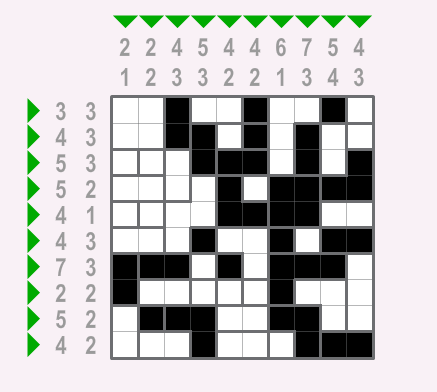
\includegraphics[scale=0.5]{res/puzzlesolved.png}
\caption{Puzzle DualClue Cross-a-Pix depois de resolvido}
\label{fig:emptypuzzle}
\end{figure}

\section{Descrição do Problema}

O DualClue Cross-a-Pix é um puzzle que consiste numa matriz M x N, dividida em várias regiões, com duas pistas em cada linha e coluna - a primeira representa o número de quadrados que estão pintados ao longo dessa linha/coluna, e a segunda representa o número de blocos (ou seja, o número de secções de quadrados pintados consecutivamente, como se pode ver na fig. \ref{fig:section}) ao longo dessa linha/coluna. Todos os quadrados de uma secção devem estar ou pintados ou não pintados.

\begin{figure}[h]
\ref{fig:emptypuzzle}
\centering
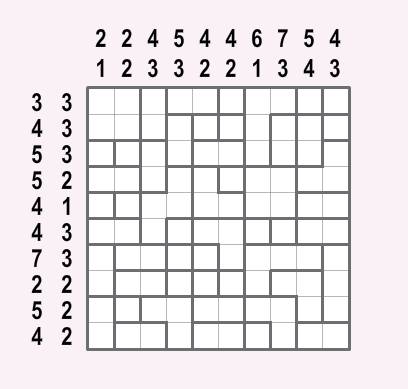
\includegraphics[scale=0.5]{res/emptypuzzle.png}
\caption{Estado do puzzle antes de ser começado. Podemos ver no topo e à esquerda as pistas dadas ao jogador}
\label{fig:emptypuzzle}
\end{figure}

\begin{figure}[h]
\ref{fig:section}
\centering
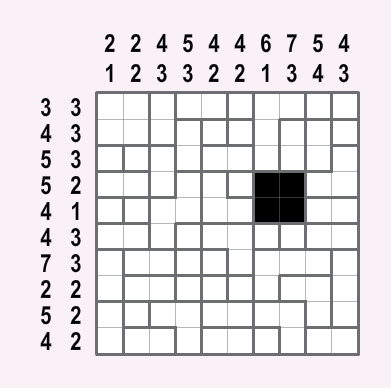
\includegraphics[scale=0.5]{res/section.png}
\caption{Uma secção}
\label{fig:section}
\end{figure}

\section{Abordagem}

Na implementação do puzzle em Prolog, optámos por representar os dados em várias estruturas de dados:

\begin{itemize}
\item Uma lista de listas, de tamanho M-1 x N-1 em que cada elemento toma o valor 0 ou 1, significando 1 ter uma parede à sua direita e 0 a sua ausência (define-se uma parede como sendo a delimitação de uma região) (definida daqui para a frente como \textbf{HP}).
\item Outra lista de listas com o mesmo tamanho, que guarda a mesma informação, mas para a existência ou não de parede em baixo (definida daqui para a frente como \textbf{VP}).
\item Uma lista de pares, em que cada par representa os números acima de cada coluna (definida daqui para a frente como \textbf{C}).
\item Uma lista de pares, em que cada par representa os números acima de cada linha (definida daqui para a frente como \textbf{L}).
\end{itemize}

\subsection{Variáveis de Decisão}

A solução é dada numa lista de listas (daqui para a frente referida como \textbf{T}). Cada lista contém informação sobre cada linha, sendo o domínio de cada lista {0,1}, sendo que 0 representa um quadrado não pintado, e 1 um quadrado pintado. O tamanho de T é, então M x N.

Apresentamos de seguida o predicado que determina a solução:

\begin{lstlisting}
doubleCrossAPixSolver(-HP, -VP, +T, -V, -H) :-	
	append(T, Vars),
	domain(Vars, 0, 1),
	groupsWithSameColour(HP,VP,T),
	horizontalRule(T,H),
	verticalRule(T,V),
	labeling([ff,enum],Vars).
\end{lstlisting}

\subsection{Restrições}

O puzzle pode ser resolvido recorrendo a 5 restrições:

\begin{enumerate}
\item Para cada elemento pertencente ao mesmo bloco, a sua cor tem de ser igual;
\item O numero de quadrados pretos de uma coluna C tem de ser igual a V[C][0];
\item O numero de blocos pretos de uma coluna C tem de ser igual a V[C][1];
\item O numero de quadrados pretos de uma linha L tem de ser igual a H[L][0];
\item O numero de blocos pretos de uma linha L tem de ser igual a H[L][1].
\end{enumerate}

\subsubsection{Para cada elemento pertencente ao mesmo bloco, a sua cor tem de ser igual}
\paragraph{}
Para cada elemento do puzzle, são testados todos os elementos na vertical e horizontal até encontrarmos uma parede - ou seja, fim do bloco. Verifica-se se têm todos a mesma cor.
Esta restrição é testada no seguinte predicado:
\paragraph{}
\begin{lstlisting}
groupsWithSameColour(-HP, -VP, +T).
\end{lstlisting}

\subsubsection{O numero de quadrados pretos de uma coluna C tem de ser igual a V[C][0] e O numero de blocos pretos de uma coluna C tem de ser igual a V[C][1]}
\paragraph{}
Percorre-se a coluna C e contam-se os quadrados pintados e as secções. Verifica-se se são iguais a V[C][0] e V[C][1], respetivamente.
Estas duas restrições são testadas no mesmo predicado, sendo este o seguinte:
\paragraph{}
\begin{lstlisting}
verticalRule(-T,+V).
\end{lstlisting}

\subsubsection{O numero de quadrados pretos de uma coluna C tem de ser igual a V[C][0] e O numero de blocos pretos de uma coluna C tem de ser igual a V[C][1]}
\paragraph{}
Percorre-se a linha L e contam-se os quadrados pintados e as secções. Verifica-se se são iguais a H[L][0] e H[L][1], respetivamente.
Estas duas restrições são testadas no mesmo predicado, sendo este o seguinte:
\paragraph{}
\begin{lstlisting}
horizontalRule(-T,+H).
\end{lstlisting}

\subsection{Estratégia de Pesquisa}

No que toca ao \textit{labeling}, usamos as seguintes estratégias:

\begin{itemize}
\item Escolha de variável:  estratégia 'ffc', que consiste na escolha da variável de menor domínio com maior número de restrições.
\item Ordenação de valores do domínio: estratégia 'up', que seleciona os valores do domínio por ordem ascendente.
\item Branching : estratégia 'enum', atribuindo sequencialmente os valores do domínio à variável.
\end{itemize}

\section{Visualização da Solução}

A solução do puzzle é mostrada no ecrã de forma simples, mas de fácil percepção. A figura \ref{fig:outputboard} mostra o resultado após o programa resolver um puzzle.

\begin{figure}[h]
\ref{fig:outputboard}
\centering
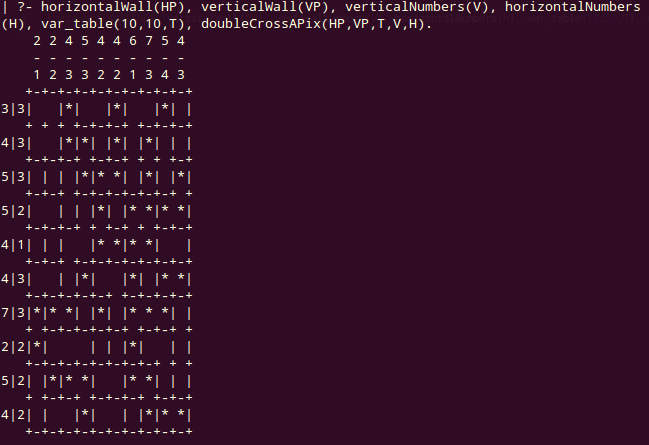
\includegraphics[scale=0.5]{res/output.png}
\caption{Output produzido no terminal para o puzzle}
\label{fig:outputboard}
\end{figure}

Para imprimir a solução, recorremos ao seguinte predicado:

\begin{lstlisting}
print_puzzle(+HP, +VP, -T, +H, +V) .
\end{lstlisting}

Em que HP, VP, T, H e V têm os significados já descritos anteriormente.

\section{Resultados}

Foram realizados vários testes para avaliar a prestação do programa, sujeitando-o a várias condições, com complexidade diferente. Para avaliar a sua prestação, recorremos ao predicado statistics/2 para determinar o tempo que decorreu entre o início e o fim da execução do teste. É importante referir que a precisão deste predicado vai até ao centésimo de segundo.

Foram feitos dois testes, um para testar o tempo necessário para gerar um puzzle e outro para testar o tempo necessário para gerar um puzzle e resolvê-lo. Implementámos dois predicados para correr estes testes, sendo eles os seguintes:

\begin{lstlisting}
assess_time_generator(-Tries, -M, -N, +Average).
assess_time_generate_and_solve(-Tries, -M, -N, +Average).
\end{lstlisting}

Apresenta-se então os testes realizados e seus resultados.

\begin{table}[]
\begin{tabular}{cccll}
\multicolumn{1}{l}{\textbf{Tamanho do Puzzle}} & \multicolumn{1}{l}{\textbf{Número de execuções}} & \multicolumn{1}{l}{\textbf{Tempo médio de execução}} &  &  \\
5x5                                            & 300                                              & 0.0011s                                               &  &  \\
10x10                                          & 300                                              & 0.0022s                                               &  &  \\
20x20                                          & 300                                              & 0.0063s                                               &  &  \\
50x50                                          & 100                                              & 0.0385s                                               &  &  \\
100x100                                        & 100                                               & 0.1724s                                               &  & 
\end{tabular}
\caption{Resultados do teste ao tempo necessário para gerar um puzzle}
\end{table}


\begin{table}[]
\centering

\begin{tabular}{cccll}
\multicolumn{1}{l}{\textbf{Tamanho do Puzzle}} & \multicolumn{1}{l}{\textbf{Número de execuções}} & \multicolumn{1}{l}{\textbf{Tempo médio de execução}} &  &  \\
5x5                                            & 100                                              & 0.0008s                                              &  &  \\
10x10                                          & 100                                              & 0.0063s                                              &  &  \\
50x50                                          & 100                                              & 0.0518s                                              &  &  \\
100x100                                        & 100                                              & 0.2143s                                              &  & 
\end{tabular}
\caption{Resultados do teste ao tempo necessário para gerar um puzzle e resolvê-lo}
\end{table}

Com isto, podemos tirar várias conclusões:

\begin{itemize}
\item O programa encontra soluções bastante rápido para puzzles com tamanho até 40x40. A partir daí, começa a demorar bastante tempo para conseguir resolver o puzzle. No entanto, tendo em conta que o número de células e regiões começa a entrar na ordem dos milhares, e as hipóteses a testar na ordem dos decaliões, tal resultado não é de estranhar.
\item O tempo para resolver um puzzle é bastante superior ao tempo para gerar um puzzle aleatório.
\item Tanto o tempo para gerar um puzzle, como o tempo para gerar um e resolvê-lo (de 2500 para 10000 células, houve um aumento de 4 vezes do tempo de execução em ambos os casos, e essa tendência é verificável também, por exemplo, de 100 para 400 células no caso da geração e resolução), aumenta de forma linear.
\end{itemize}

\section{Conclusões}
Contrariamente ao projeto anterior, não foi preciso tanto tempo para concluir este. No entanto, não é por isso que deixámos de cumprir o principal objetivo de consolidar os conhecimentos referentes à programação em lógica com restrições.

O uso de restrições não só vem facilitar bastante a resolução de problemas como o DualClue Cross-a-Pix, como o faz de forma extremamente rápida e eficiente. Depois de compreendido, o grupo considera este um conceito extremamente interessante de colocar em prática, e o facto de o puzzle ser bastante cativante tornou a realização deste projeto uma experiência bastante agradável. 

\section*{Anexo}

\subsection*{Código fonte}
\lstinputlisting[language=Prolog, breaklines=true]{../crossapix.pl}

\end{document}